
\section{Séance 2}

\begin{exo}
Consid\'erez la grille $n \times n$, le graphe obtenu selon la Figure~\ref{fig:grille}, avec $n$ un naturel~$\geq 3$.
D\'emontrez que $n$ est pair si et seulement si le graphe est hamiltonien.
\end{exo}

\input{TP2/Figures/Grille.tikz}

Nous cherchons à prouver que tout graphe du style de la figure \ref{fig:grille} avec un n pair est un graphe hamiltonien. C'est à dire n pair $\Leftrightarrow$ graphe hamiltonien.

$\Leftarrow$ Si n est impair, alors $n=2k + 1$ et le graphe a $n^2 = (2k + 1)^2 = 4k^2 + 4k + 1$ sommets, c'est à dire un nombre impair de sommets.

Or, le graphe est biparti (via les diagonales).

\input{TP2/Figures/GrilleBicolore.tikz}

Si le graphe est hamiltonien, cela veut dire qu'il contient un cycle d'ordre impair, ce qui contredit G biparti.

$\Rightarrow$ Démontrons par récurrence sur $2n \geq 4$ que la grille contient un cycle hamiltonien contenant une arête spécifique (pour nous faciliter la tâche) que l'on nommera ``E''.

\textbf{Cas de base n=4: } OK

\begin{figure}[!h]
\centering
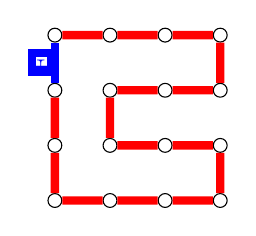
\begin{tikzpicture}[scale = 0.70]

\node[circle, draw, fill=white, inner sep=0pt, minimum size=5pt] (v16) at (0,0) {};
\node[circle, draw, fill=white, inner sep=0pt, minimum size=5pt] (v9) at (1,0) {};
\node[circle, draw, fill=white, inner sep=0pt, minimum size=5pt] (v10) at (2,0) {};
\node[circle, draw, fill=white, inner sep=0pt, minimum size=5pt] (v11) at (3,0) {};
\node[circle, draw, fill=white, inner sep=0pt, minimum size=5pt] (v1) at (0,-1) {};
\node[circle, draw, fill=white, inner sep=0pt, minimum size=5pt] (v8) at (0,-2) {};
\node[circle, draw, fill=white, inner sep=0pt, minimum size=5pt] (v7) at (0,-3) {};
\node[circle, draw, fill=white, inner sep=0pt, minimum size=5pt] (v12) at (3,-1) {};
\node[circle, draw, fill=white, inner sep=0pt, minimum size=5pt] (v3) at (3,-2) {};
\node[circle, draw, fill=white, inner sep=0pt, minimum size=5pt] (v4) at (3,-3) {};
\node[circle, draw, fill=white, inner sep=0pt, minimum size=5pt] (v6) at (1,-3) {};
\node[circle, draw, fill=white, inner sep=0pt, minimum size=5pt] (v5) at (2,-3) {};
\node[circle, draw, fill=white, inner sep=0pt, minimum size=5pt] (v14) at (1,-1) {};
\node[circle, draw, fill=white, inner sep=0pt, minimum size=5pt] (v13) at (2,-1) {};
\node[circle, draw, fill=white, inner sep=0pt, minimum size=5pt] (v15) at (1,-2) {};
\node[circle, draw, fill=white, inner sep=0pt, minimum size=5pt] (v2) at (2,-2) {};

\draw[red,,line width=3pt] (v15) -- (v2) -- (v3) -- (v4) -- (v5) -- (v6) -- (v7) -- (v8) -- (v1);
\draw[red,,line width=3pt] (v16) -- (v9) -- (v10) -- (v11) -- (v12) -- (v13) -- (v14) -- (v15);
\draw[blue,,line width=3pt]  (v1) edge node[sloped, above] {E} (v16);


\end{tikzpicture}
\end{figure}

\textbf{Étape d'induction}

\begin{figure}[!h]
\centering
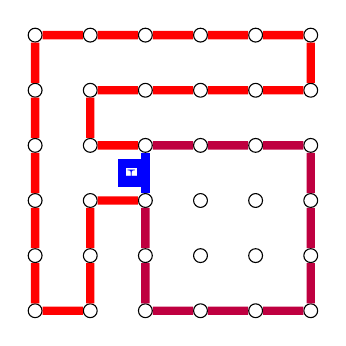
\begin{tikzpicture}[scale = 0.70]

\node[circle, draw, fill=white, inner sep=0pt, minimum size=5pt] (v11) at (0,0) {};
\node[circle, draw, fill=white, inner sep=0pt, minimum size=5pt] (v10) at (1,0) {};
\node[circle, draw, fill=white, inner sep=0pt, minimum size=5pt] (v9) at (2,0) {};
\node[circle, draw, fill=white, inner sep=0pt, minimum size=5pt] (v8) at (3,0) {};
\node[circle, draw, fill=white, inner sep=0pt, minimum size=5pt] (vX) at (3,-1) {};
\node[circle, draw, fill=white, inner sep=0pt, minimum size=5pt] at (2,-1) {};
\node[circle, draw, fill=white, inner sep=0pt, minimum size=5pt] at (1,-1) {};
\node[circle, draw, fill=white, inner sep=0pt, minimum size=5pt] (v1) at (0,-1) {};
\node[circle, draw, fill=white, inner sep=0pt, minimum size=5pt] (v2) at (0,-2) {};
\node[circle, draw, fill=white, inner sep=0pt, minimum size=5pt] at (1,-2) {};
\node[circle, draw, fill=white, inner sep=0pt, minimum size=5pt] at (2,-2) {};
\node[circle, draw, fill=white, inner sep=0pt, minimum size=5pt] (v7) at (3,-2) {};
\node[circle, draw, fill=white, inner sep=0pt, minimum size=5pt] (v6) at (3,-3) {};
\node[circle, draw, fill=white, inner sep=0pt, minimum size=5pt] (v5) at (2,-3) {};
\node[circle, draw, fill=white, inner sep=0pt, minimum size=5pt] (v4) at (1,-3) {};
\node[circle, draw, fill=white, inner sep=0pt, minimum size=5pt] (v3) at (0,-3) {};
\node[circle, draw, fill=white, inner sep=0pt, minimum size=5pt] (v17) at (3,1) {};
\node[circle, draw, fill=white, inner sep=0pt, minimum size=5pt] (v18) at (3,2) {};
\node[circle, draw, fill=white, inner sep=0pt, minimum size=5pt] (v16) at (2,1) {};
\node[circle, draw, fill=white, inner sep=0pt, minimum size=5pt] (v19) at (2,2) {};
\node[circle, draw, fill=white, inner sep=0pt, minimum size=5pt] (v15) at (1,1) {};
\node[circle, draw, fill=white, inner sep=0pt, minimum size=5pt] (v20) at (1,2) {};
\node[circle, draw, fill=white, inner sep=0pt, minimum size=5pt] (v14) at (0,1) {};
\node[circle, draw, fill=white, inner sep=0pt, minimum size=5pt] (v21) at (0,2) {};
\node[circle, draw, fill=white, inner sep=0pt, minimum size=5pt] (v12) at (-1,0) {};
\node[circle, draw, fill=white, inner sep=0pt, minimum size=5pt] (v31) at (-1,-1) {};
\node[circle, draw, fill=white, inner sep=0pt, minimum size=5pt] (v30) at (-1,-2) {};
\node[circle, draw, fill=white, inner sep=0pt, minimum size=5pt] (v29) at (-1,-3) {};
\node[circle, draw, fill=white, inner sep=0pt, minimum size=5pt] (v28) at (-2,-3) {};
\node[circle, draw, fill=white, inner sep=0pt, minimum size=5pt] (v27) at (-2,-2) {};
\node[circle, draw, fill=white, inner sep=0pt, minimum size=5pt] (v26) at (-2,-1) {};
\node[circle, draw, fill=white, inner sep=0pt, minimum size=5pt] (v25) at (-2,0) {};
\node[circle, draw, fill=white, inner sep=0pt, minimum size=5pt] (v13) at (-1,1) {};
\node[circle, draw, fill=white, inner sep=0pt, minimum size=5pt] (v22) at (-1,2) {};
\node[circle, draw, fill=white, inner sep=0pt, minimum size=5pt] (v23) at (-2,2) {};
\node[circle, draw, fill=white, inner sep=0pt, minimum size=5pt] (v24) at (-2,1) {};

\draw[purple,line width=3pt] (v1) -- (v2) -- (v3) -- (v4) -- (v5) -- (v6) -- (v7) -- (vX) -- (v8) -- (v9) -- (v10) -- (v11);

\draw[blue,line width=3pt]  (v1) edge node[sloped, above] {E} (v11);

\draw[red,line width=3pt] (v11) -- (v12) -- (v13) -- (v14) -- (v15) -- (v16) -- (v17) -- (v18) -- (v19) -- (v20) -- (v21) -- (v22) -- (v23) -- (v24) -- (v25) -- (v26) -- (v27) -- (v28) -- (v29) -- (v30) -- (v31) -- (v1);

\end{tikzpicture}
\end{figure}

Dans la grille $(2n+2) \times (2n+2)$, nous avons une sous-grille (en mauve) qui est de taille $2n \times 2n$. Par hypothèse d'induction, il existe un cycle hamiltonien contenant l'arête E. Dans ce cycle, si on élimine l'arête E et on rajoute le chemin en rouge (qui est composé des sommets ``+2''), nous obtenons un cycle hamiltonien.

\newpage
%-----------------------------------------------------------------

\begin{exo}
Prouvez que pour tout $n \geq 3$, le graphe complet $K_n$ poss\`ede exactement $\frac{1}{2}(n-1)!$ cycles hamiltoniens.
\end{exo}

\textbf{Cas de base} n=3, il s'agit d'un triangle. Ce graphe a $\frac{1}{2}(3-1)! = 1$ cycle hamiltonien.

\textbf{Récurrence} Supposons vrai pour $K_n$. Nous savons donc que $K_n$ possède $\frac{1}{2}(n-1)!$ cycles hamiltoniens. 

Pour $K_{n+1}$, nous construisons n cycles hamiltoniens supplémentaires en ajoutant le nouveau sommet entre 2 sommets quelconques de chaque cycle.

Donc, pour $K_{n+1}$ nous avons $\frac{1}{2}(n-1)!n = \frac{1}{2}n!$ cycles hamiltoniens.


%-----------------------------------------------------------------

\begin{exo}
Combien d'arbres couvrants poss\`edent les deux graphes de la Figure~\ref{fig:arbrecouvrant}?
\end{exo}

\begin{figure}[!h]
\centering
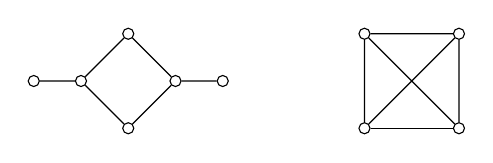
\begin{tikzpicture}[scale = 0.6]
\tikzstyle{every node}=[draw,circle,fill=black,minimum size=4pt,inner sep=0pt]
\node (a1) at (0,0) [shape= circle, draw, fill = white] {};
\node (a2) at (1,0) [shape= circle, draw, fill = white] {};
\node (a3) at (2,1) [shape= circle, draw, fill = white] {};
\node (a4) at (3,0) [shape= circle, draw, fill = white] {};
\node (a5) at (4,0) [shape= circle, draw, fill = white] {};
\node (a6) at (2,-1) [shape= circle, draw, fill = white] {};
\draw (a1) -- (a2) -- (a3) -- (a4) -- (a5);
\draw (a2) -- (a6) -- (a4);

\node (b1) at (7,-1) [shape= circle, draw, fill = white] {};
\node (b2) at (9,-1) [shape= circle, draw, fill = white] {};
%\node (b3) at (10,0) [shape= circle, draw, fill = white] {};
\node (b4) at (9,1) [shape= circle, draw, fill = white] {};
\node (b5) at (7,1) [shape= circle, draw, fill = white] {};
\draw (b1) -- (b2); -- (b3) -- 
\draw (b4) -- (b5) -- (b1) -- (b4) -- (b2) -- (b5);
\end{tikzpicture}
\caption{}
\label{fig:arbrecouvrant}
\end{figure}

\textbf{Graphe de gauche:} Il existe 4 arbres couvrants

\begin{figure}[!h]
\centering
\scalebox{.825}{\begin{tikzpicture}

\tikzstyle{every node}=[circle, draw, fill=white, inner sep=0pt, minimum size=5pt]

\node (v1) at (0,0) {};
\node (v2) at (1,0) {};
\node (v3) at (2,1) {};
\node (v4) at (3,0) {};
\node (v6) at (2,-1) {};
\node (v5) at (4,0) {};
\draw (v1) -- (v2) -- (v3) -- (v4) -- (v5);
\draw  (v6) edge (v4);
\node (v9) at (7,1) {};
\node (v12) at (7,-1) {};
\node (v10) at (8,0) {};
\node (v11) at (9,0) {};
\node (v8) at (6,0) {};
\node (v7) at (5,0) {};
\node (v18) at (12,1) {};
\node (v15) at (12,-1) {};
\node (v14) at (13,0) {};
\node (v13) at (14,0) {};
\node (v16) at (11,0) {};
\node (v17) at (10,0) {};
\node (v24) at (17,1) {};
\node (v21) at (17,-1) {};
\node (v22) at (18,0) {};
\node (v23) at (19,0) {};
\node (v20) at (16,0) {};
\node (v19) at (15,0) {};
\draw (v7) -- (v8) -- (v9) -- (v10) -- (v11);
\draw  (v12) edge (v8);
\draw (v13) -- (v14) -- (v15) -- (v16) -- (v17);
\draw  (v18) edge (v16);
\draw (v19) -- (v20) -- (v21) -- (v22) -- (v23);
\draw  (v22) edge (v24);
\end{tikzpicture}}
\end{figure}

\textbf{Graphe de droite:} Il existe 16 arbres couvrants. Trop nombreux pour que je les dessine tous.


%-----------------------------------------------------------------

\begin{exo}
Montrez que tous les alcools $C_nH_{2n+1}OH$ sont des mol\'ecules dont le graphe est un arbre, en sachant que les valences de $C, O$ et de $H$ sont respectivement $4, 2, 1$.
\end{exo}

\[ \sum_{v\in V} deg(v) = (n\cdot 4) + (2n + 1)\cdot 1 + (1\cdot 2) + (1\cdot 1) = 6n + 4 = 2(3n + 2) \]

Donc, $ |E| = 3n + 2$. Or, $|V| = 3n + 3$. Or, G connexe. $\Rightarrow$ G est un arbre.

\begin{figure}[htb]
	\centering
	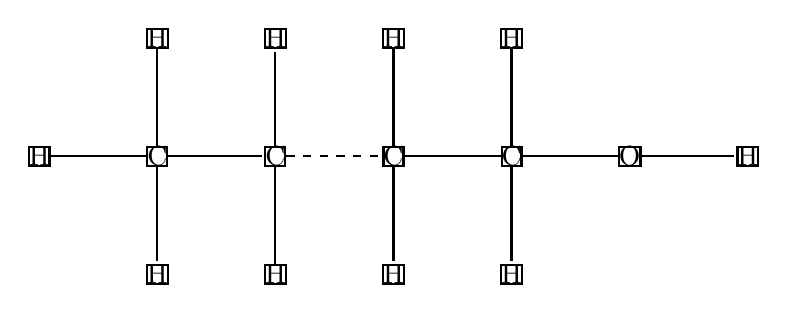
\begin{tikzpicture}[shorten >=1pt,auto,node distance=1.5cm,thick]

	\node (c1) {C};
	\node (c2) [right of=c1] {C};
	\node (h1) [above of=c1] {H};
	\node (h2) [left of=c1] {H};
	\node (h3) [below of=c1] {H};
	\node (h4) [above of=c2] {H};
	\node (h5) [below of=c2] {H};

	\node (c3) [right of=c2] {C};
	\node (c4) [right of=c3] {C};
	\node (h6) [above of=c3] {H};
	\node (h7) [below of=c3] {H};
	\node (h8) [above of=c4] {H};
	\node (h9) [below of=c4] {H};

	\node (o) [right of=c4] {O};
	\node (hX) [right of=o] {H};

	\draw (h2) -- (c1) -- (c2);
	\draw (c3) -- (c4) -- (o) -- (hX);

	\draw[dashed] (c2) -- (c3);

	\draw (h1) -- (c1) -- (h3);
	\draw (h5) -- (c2) -- (h4);
	\draw (h6) -- (c3) -- (h7);
	\draw (h8) -- (c4) -- (h9);

	\end{tikzpicture}

\end{figure}

Les graphes correspondants sont des arbres, avec la molécule 0 comme racine, et à sa gauche et droite les sous-arbres.

\newpage

%-----------------------------------------------------------------

\begin{exo}
D\'emontrez que si un graphe hamiltonien $G = (V,E)$ est biparti selon la bipartition $V = A \cup B$, alors $|A|= |B|$. En d\'eduire que $K_{n,m}$, le graphe biparti complet, est hamiltonien si et seulement si $m=n \geq 2$.

\end{exo}

<MISSING>

%-----------------------------------------------------------------

\begin{exo}
Pour chaque graphe de la Figure~\ref{fig:graphes}, d\'eterminez si 
\begin{enumerate}
\item le graphe est hamiltonien,
\item le graphe est eul\'erien,
\item le graphe est biparti.
\end{enumerate}
\end{exo}

\begin{figure}[!h]
\centering
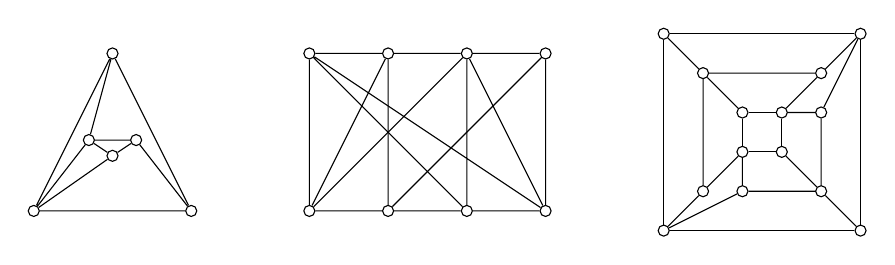
\begin{tikzpicture}[scale = 0.5]
\tikzstyle{every node}=[draw,circle,fill=black,minimum size=4pt,inner sep=0pt]
\node (a1) at (0,4) [shape= circle, draw, fill = white] {};
\node (a2) at (-2,0) [shape= circle, draw, fill = white] {};
\node (a3) at (2,0) [shape= circle, draw, fill = white] {};
\node (a4) at (0.6,1.8) [shape= circle, draw, fill = white] {};
\node (a5) at (-0.6,1.8) [shape= circle, draw, fill = white] {};
\node (a6) at (0,1.4) [shape= circle, draw, fill = white] {};
\draw (a1) -- (a2) -- (a3) -- (a1) -- (a5) -- (a2);
\draw (a2) -- (a6) -- (a4);
\draw (a3) -- (a4) -- (a5) -- (a6);

\node (a1) at (5,0) [shape= circle, draw, fill = white] {};
\node (a2) at (7,0) [shape= circle, draw, fill = white] {};
\node (a3) at (9,0) [shape= circle, draw, fill = white] {};
\node (a4) at (11,0) [shape= circle, draw, fill = white] {};
\node (b1) at (5,4) [shape= circle, draw, fill = white] {};
\node (b2) at (7,4) [shape= circle, draw, fill = white] {};
\node (b3) at (9,4) [shape= circle, draw, fill = white] {};
\node (b4) at (11,4) [shape= circle, draw, fill = white] {};
\draw (a1) -- (a2) -- (a3) -- (a4) -- (b4) -- (b3) -- (b2) -- (b1) -- (a1) -- (b2);
\draw (a1) -- (b3) -- (a4) -- (b1) -- (a3) -- (b3) ;
\draw (b2) -- (a2) -- (b4);


\node (a1) at (14,-0.5) [shape= circle, draw, fill = white] {};
\node (a2) at (14,4.5) [shape= circle, draw, fill = white] {};
\node (a3) at (19,4.5) [shape= circle, draw, fill = white] {};
\node (a4) at (19,-0.5) [shape= circle, draw, fill = white] {};

\node (b1) at (15,0.5) [shape= circle, draw, fill = white] {};
\node (b11) at (16,0.5) [shape= circle, draw, fill = white] {};
\node (b2) at (15,3.5) [shape= circle, draw, fill = white] {};
\node (b33) at (18,2.5) [shape= circle, draw, fill = white] {};
\node (b3) at (18,3.5) [shape= circle, draw, fill = white] {};
\node (b4) at (18,0.5) [shape= circle, draw, fill = white] {};

\node (c1) at (16,1.5) [shape= circle, draw, fill = white] {};
\node (c2) at (16,2.5) [shape= circle, draw, fill = white] {};
\node (c3) at (17,2.5) [shape= circle, draw, fill = white] {};
\node (c4) at (17,1.5) [shape= circle, draw, fill = white] {};

\draw (a1) -- (a2) -- (a3) -- (a4) -- (a1);
\draw (a1) -- (b1) -- (b2) -- (b3) -- (a3);
\draw (a1) -- (b11) -- (b4) -- (b33) -- (a3);
\draw (a2) -- (b2) -- (c2);
\draw (a4) -- (b4) -- (c4);
\draw (c1) -- (c2) -- (c3) -- (c4) -- (c1);
\draw (b1) -- (c1) -- (b11);
\draw (b33) -- (c3) -- (b3);
\end{tikzpicture}
\caption{}
\label{fig:graphes}
\end{figure}


\textbf{Graphe 1:} Hamiltonien (voir chemin rouge). Non-eulérien ($deg(v_1)=3$). Non-biparti car $K_3$.

\textbf{Graphe 2:} Hamiltonien (voir chemin rouge). Non-eulérien ($deg(v_2)=3$). Non-biparti car $K_3$.

\textbf{Graphe 3:} Non-hamiltonien car $|A| \neq |B|$. Non-eulérien ($deg(v_3)=3$). Biparti.

\begin{figure}[!h]
\centering
\begin{tikzpicture}[scale = 0.8]

\tikzstyle{every node}=[draw,minimum size=4pt,inner sep=0pt]

\node (a1) at (0,4) [shape= circle, draw, fill = white,label={[label distance=1cm]},label=$v_1$] {};
\node (a2) at (-2,0) [shape= circle, draw, fill = white] {};
\node (a3) at (2,0) [shape= circle, draw, fill = white] {};
\node (a4) at (0.6,1.8) [shape= circle, draw, fill = white] {};
\node (a5) at (-0.6,1.8) [shape= circle, draw, fill = white] {};
\node (a6) at (0,1.4) [shape= circle, draw, fill = white] {};
\draw[red,line width=2pt] (a2) -- (a1) -- (a3) -- (a4) -- (a6) -- (a5) -- (a2) -- (a1);
\draw (a1) -- (a5) -- (a4);
\draw (a6) -- (a2) -- (a3);

\node (a1) at (5,0) [shape= circle, draw, fill = white] {};
\node (a2) at (7,0) [shape= circle, draw, fill = white] {};
\node (a3) at (9,0) [shape= circle, draw, fill = white] {};
\node (a4) at (11,0) [shape= circle, draw, fill = white] {};
\node (b1) at (5,4) [shape= circle, draw, fill = white] {};
\node (b2) at (7,4) [shape= circle, draw, fill = white] {};
\node (b3) at (9,4) [shape= circle, draw, fill = white] {};
\node (b4) at (11,4) [shape= circle, draw, fill = white,label={[label distance=1cm]},label=$v_2$] {};
\draw[red,line width=2pt] (a1) -- (a2) -- (a3) -- (a4) -- (b4) -- (b3) -- (b2) -- (b1) -- (a1);
\draw (a1) -- (b3) -- (a4) -- (b1) -- (a3) -- (b3) ;
\draw (b2) -- (a2) -- (b4);
\draw (a1) -- (b2);


\node (a1) at (14,-0.5) [shape= circle, draw, fill = red] {};
\node (a2) at (14,4.5) [shape= circle, draw, fill = blue] {};
\node (a3) at (19,4.5) [shape= circle, draw, fill = red] {};
\node (a4) at (19,-0.5) [shape= circle, draw, fill = blue] {};
\node [below right = 0.2 cm and 0.2 cm of a4, draw=none,fill=none](everynode){$v_3$};

\node (b1) at (15,0.5) [shape= circle, draw, fill = blue] {};
\node (b11) at (16,0.5) [shape= circle, draw, fill = blue] {};
\node (b2) at (15,3.5) [shape= circle, draw, fill = red] {};
\node (b33) at (18,2.5) [shape= circle, draw, fill = blue] {};
\node (b3) at (18,3.5) [shape= circle, draw, fill = blue] {};
\node (b4) at (18,0.5) [shape= circle, draw, fill = red] {};

\node (c1) at (16,1.5) [shape= circle, draw, fill = red] {};
\node (c2) at (16,2.5) [shape= circle, draw, fill = blue] {};
\node (c3) at (17,2.5) [shape= circle, draw, fill = red] {};
\node (c4) at (17,1.5) [shape= circle, draw, fill = blue] {};

\draw (a1) -- (a2) -- (a3) -- (a4) -- (a1);
\draw (a1) -- (b1) -- (b2) -- (b3) -- (a3);
\draw (a1) -- (b11) -- (b4) -- (b33) -- (a3);
\draw (a2) -- (b2) -- (c2);
\draw (a4) -- (b4) -- (c4);
\draw (c1) -- (c2) -- (c3) -- (c4) -- (c1);
\draw (b1) -- (c1) -- (b11);
\draw (b33) -- (c3) -- (b3);
\end{tikzpicture}
\end{figure}

%-----------------------------------------------------------------

